\chapter{Coatings for ATHENA}\label{chap:athena_coatings}


\section{Investigating the baseline Ir/B$_4$C coating}
\section{Film stress}
\begin{figure}[htbp]
  \centering
    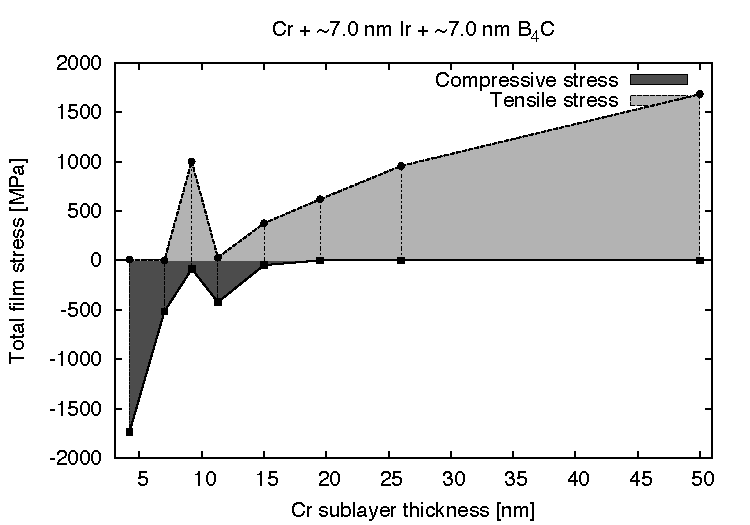
\includegraphics[height=6cm]{figures/athena/stress_ir_b4c.pdf}
  \caption{}
  \label{fig:stress_irb4c}
\end{figure}

\section{Alternative coatings}
\section{Findings from long term storage}
\section{Novel coating methods}
\subsection{Pulsed-DC sputtering}

\subsection{Reactive sputtering with N$_2$}

\section{Upscaled production}

\emph{The following section was part of a technical report for the European Space Agency. It was done as part of the coating investigations for ATHENA+, which was had a double-telescope configuration. It also required significantly less silicon port optic substrates, 64,640 vs. $\sim$300,000 for ATHENA. The investigations done for scaling up production still holds true and the final production will also still take 2 years, but cost and production equipment and man-power will have to increase by a factor of four to five.}

For the ATHENA mission, the coating of the mirror substrates will be a large undertaking as 64,640 silicon pore optic (SPO) substrates will need a coating of between two and twenty layers.

Every piece will have to be transported from the SPO substrate fabrication facility (SFF) to a new dedicated coating facility, thoroughly cleaned, coated in specially designed chambers transported to the stacking facility. After stacking into mirror modules (MM), each MM will be measured at one of three dedicated beam lines at the BESSY II synchrotron in Berlin.

In this paper, an approximate cost timeline of the coating qualification of SPO substrates is given.

\subsection{Timeline cost of procurement setup of coating facility}

Cleaning coating of SPO substrates will require as a minimum an ISO 7 clean room to avoid dust particles. Dust on the substrates before coating will result in small holes in the coating, which will reduce the effective area. There are two possibilities for the location of the coating facility which is discussed in this paper. Either the facility is located in the same building or adjacent building as the stacking facility or the coating facility is placed further away, i.e. another country.

Moving substrates in out of clean rooms transporting them over larger distances has drawbacks extra costs associated. But locating the two facilities separately can reduce costs as it will be easier cheaper to find two smaller clean rooms to repurpose into production facilities. Building setting up a clean rooms of a sufficient size for both facilities will take several years come with a significant cost, but if it is possible to repurpose existing laboratories that cost can be reduced.

The first part of the clean room should be for opening shipments from the SFF cleaning each substrate. As the substrates are produced in a clean room at the SFF, it is assumed that they will at maximum need to be cleaned with an air gun with dry nitrogen. After being cleaned, each substrate is mounted onto a substrate holder that will be inserted into a coating chamber for coating. When the coating is done, the substrate holder is taken out of the chamber and the substrates are ready to go into the stacking facility.

Clean rooms can be build inside existing larger storage areas or cleaner production facilities. The approximate timeline for the setup of the entire facility is as follows:

\begin{description}[itemsep=1.5pt,parsep=1pt]
	\item[9] \textbf{years before launch:}
		\begin{itemize}[itemsep=1.5pt,parsep=1pt]
		\item[-] Planning is begun for the construction of a shared cleanroom facility
		\item[-] Planning is begun for coating chambers
		\end{itemize}
	\item[7-8] \textbf{years before launch:}
		\begin{itemize}[itemsep=1.5pt,parsep=1pt]
		\item[-] Construction of facility is carried out.
		\item[-] Produced coating chambers are installed qualifications begun.
		\end{itemize}
	\item[6] \textbf{years before launch (CDR):}
		\begin{itemize}[itemsep=1.5pt,parsep=1pt]
		\item[-] Coating capabilities ready.
		\end{itemize}
\end{description}

The cost of building and preparing the coating facility will differ between a shared facility and separated facilities, but the coating chambers will have a similar configuration.

\subsection{Coating chambers}\label{sec:chambers}
The two telescopes of ATHENA consists of 66,640 SPO substrates, which are all coated. Considering the coating chamber design used at DTU Space, a maximum of 100 plates can be coated per day in an 8 hour workday. In a year of 200 workdays, 20,000 substrates can be coated. Using three chambers, 60,000 substrates can be coated per year, within the two year time frame a total of 120,000 substrates can be coated. A minimum of 90,000 coated is considered as baseline, as we account for damaged plates, bad coatings etc. That leaves an acceptable down time of 6 months throughout the project.

Using chambers of same design as DTU Space will give a cost of around 1M \euro per chamber. Those chambers have the drawback of a long pump down time after having the chamber opened to change samples. The advantage of coating SPO substrates compared to e.g. NuSTAR glass is that the SPO substrates are flat only $\sim$1 mm thin.

If a new chamber design is considered, it would be advantageous to pursue a design similar to what is used in the semiconductor industry. Here entire wafer are given a number of different coatings automatically moved from one cathode to another using a robotic arm. As those wafers can have a thickness of up to 3 mm, we propose to use a substrate holder shaped like a wafer 3 mm thick with a diameter of 300 mm. Recessions in the substrate holder can accommodate SPO substrate no clips will be needed to hold substrates in place, since the wafer will at all times be horizontal. A chamber of that design will not need pump down time between each batch of substrates, since wafers will be inserted into the central vacuum chamber through a narrow slit directly from a clean magazine in atmospheric pressure. Every coating cathode is also in a separate chamber can be accessed without venting the entire machine. Custom made machines like seen in figure \ref{fig:dram} are priced at $\sim$2M \euro.

\begin{figure}[htbp]
	\centering
		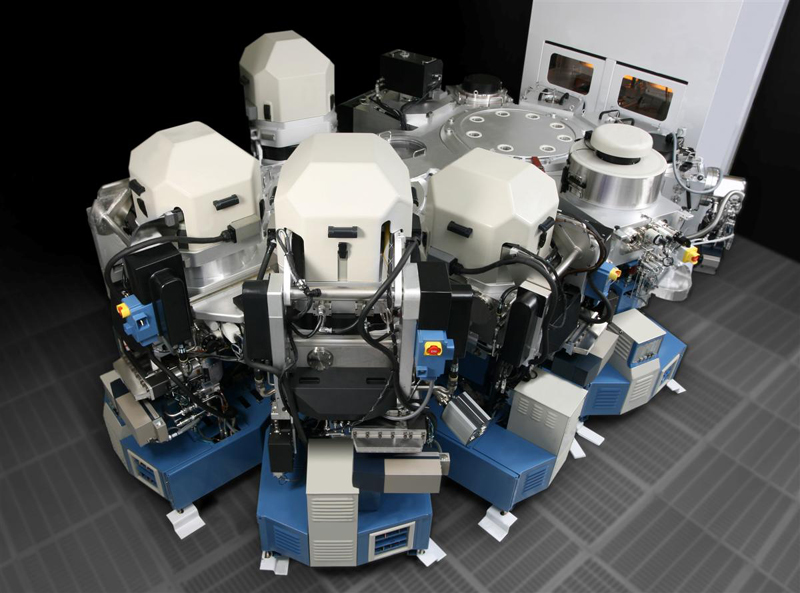
\includegraphics[width=0.6\textwidth]{figures/athena/dram.jpeg}
	\caption{Multi-chamber deposition machine from Applied Materials. \emph{Source: www.appliedmaterials.com}}
	\label{fig:dram}
\end{figure}

A significant increase production rates can be achieved using machines like this as well as a cleaner environment for samples, since the machine itself can stay closed for longer periods of time. Higher production rates means that only one or two chambers are needed to complete the coating of 90,000 SPO substrates in two years.

\subsection{Shared facility}
Since both the coating facility stacking facility needs a clean room, these can be combined or connected in a shared facility. If the chamber design from DTU Space is used, a separate clean room will be needed to accommodate these chambers as they can give off dust flakes of material every time they are opened. If instead a multi-chamber coating system is used as described in section \ref{sec:chambers}, the coating machinery can be in a separate clean room against the wall into the stacking facility. That way wafer cassettes full of wafer-shaped SPO substrate holders can be inserted retrieved from the stacking facility clean room.

For a shared facility with multi-chamber coating systems as described in section \ref{sec:chambers}, we propose the following facility setup:

\begin{itemize}
	\item Common class 10,000 clean room for mounting SPO substrates on wafer-shaped sample holders. The same room will be used for fast X-ray system for pre- post coating measurements.
	\item Access to insertion port of multi-chamber coating system from the common clean room. Wafer casettes are mounted directly to accessible part of the machine.
	\item The back end of the coating chambers are in a separate room, so targets can be changed without giving off dust near the substrates.
	\item In connection to the common clean room is a separate class 100 - 10,000 clean room with stacking robots. The robots can be in a separate ventilated tent inside the clean room to decrease particle dust. Mirror modules will be sealed here moved outside the clean rooms for packing shipping to BESSY II.
\end{itemize}

\subsection{Separated facilites}
If the facilities are separated, a large effort will be required to keep substrates clean when packing/unpacking for transport. The substrates will be send from the SFF in batches of 1,500 double or triple sealed, so the package can be opened partly when inside a moderately clean room opened completely in the main class 10,000 clean room. The following setup of clean rooms is proposed.

\begin{itemize}
	\item Two separate class 10,000 clean rooms, one for substrate handling one for coating chambers. Alternatively, one larger clean room parted by a clear plastic curtain.
	\item Substrate handling clean room will also be used for the fast X-ray system for pre- post coating measurements.
	\item Coated samples will be packed double sealed inside the clean room before being shipped to the stacking facility.
\end{itemize}

\subsection{Resist deposition removal at alternative facility}
One of the processes done at the SFF to the substrates before sending them to the coating facility will be the lithographic process of resist deposition. It requires a semiconductor grade facility to apply the resist using spray-on afterwards removing stripes by a UV radiation process.

The process can, instead of at the SFF, be done either at the coating facility by including the proper equipment or at an external facility. DTU Danchip is the Danish National Center for Micro- Nanofabrication, which runs a class 10 clean room with equipment capable of depositing the resist UV curing the SPO substrates.

The removal of the resist after coating can be done at the stacking facility, but can instead be done at the coating facility if these are separated. By doing the resist removal at the coating facility, a visual inspection can be done of the substrate before being transported to the stacking facility. If the process damages the coating, the problem can be located new coated substrates can be produced quickly.


\subsection{Cost for setting up}
To prepare the lab before the coating campaign starts, the coating chambers will need to be installed configured. An extensive campaign with scientific personnel is needed to ensure the system's capability to produce coatings of sufficient quality. We estimate 12-24 months to qualify the coating chambers for the ATHENA coating campaign will need approximately two scientific personnel one technician.

The coating qualification equipment described in section \ref{qualification} will be needed to qualify the coating chambers.


\begin{table}[htbp]
	\centering
\begin{tabular}{l|c}
Equipment & Approx. price \\
\hline
\hline
3 x Coating chambers of DTU design  & 3 x 1,000,000 \euro\\
\hline
or:\\
\hline
2 x Multi-chamber coating systems & 2 x 2,000,000 \euro \\
\hline
\\
\hline
Personnel for setup & 490,000 \euro\\
\end{tabular}
\end{table}


\subsection{Timeline cost for production of ATHENA coatings}
SPO substrates are fabricated at the SFF should be shipped to the coating facility weekly in shipments of 1500 substrates. 300 substrates are daily mounted on wafer shaped sample holders after they have been measured using the fast X-ray system. The substrates are coated in one of the coating chambers subsequently taken out to have resist removed be measured again using the fast X-ray system.

Cost drivers during production are sputtering targets personnel. The final cost is dependent on which material combination is used for coating. The differences can be seen below.

\begin{table}[htbp]
	\centering
\begin{tabular}{l|c|c|c|c}
Material 	& High Z 		& Approximate & Low Z  & Approximate \\
combination & thickness & price / mm$^3$ & thickness &  price / mm$^3$ \\
 & (nm) & (High Z) & (nm) &  (Low Z) \\
\hline
\hline
Cr/Ir/B$_4$C & 10 & 10.9 \euro & 8 & 0.26 \euro\\
\hline
Pt/B$_4$C & $\sim$16 & 10.5 \euro & $\sim$22 & 0.26 \euro\\
\hline
W/B$_4$C & $\sim$16 & 0.73 \euro & $\sim$22 & 0.26 \euro\\
\end{tabular}
\end{table}

The approximate cost is calculated based on a 10\% efficiency of the sputtering cathodes, meaning 10\% of the target material ends on a substrate. For a single layer of 10 nm on all the substrates of ATHENA, the volume of material needed will be approximately 5 cm$^3 = $ 5000 mm$^3$. From that, the total target cost can be estimated.

\begin{table}[htbp]
	\centering
\begin{tabular}{l|l|c|c}
Material 	& Type of coating & Approx. cost & Approx cost incl. \\
combination	&	&	&	30 \% target \\
&	&	&	usability\\
\hline
\hline
Cr/Ir/B$_4$C & Tri-layer & 57,000 \euro & 190,000 \euro \\
\hline
Pt/B$_4$C & Graded-d multilayer & 87,000 \euro & 290,000 \euro\\
\hline
W/B$_4$C & Graded-d multilayer & 8,700 \euro & 29,000 \euro \\
\end{tabular}
\end{table}

Only 30\% of the target can be used before it has to be replaced, so a factor of 3-4 should be applied to these cost estimates. The leftover targets of precious metals, platinum iridium, can be sold back at market value, which can reduce the total costs of precious metal consumption by up to $\sim$50 \%.

For a Pt/B$_4$C graded-d multilayer, the total thickness of Pt is 16 nm in average 22 nm of B$_4$C. Thus, $1.6 \cdot 5000$ mm$^3$ of Pt is needed at a price of 10.5 \euro per mm$^3$ at 90 \% coating loss, combined with $2.2 \cdot 5000$ mm$^3$ of B$_4$C at 0.26 \euro per mm$^3$ gives a total cost of 87,000 \euro.

\subsection{Personnel}
During the two year coating campaign, 300 substrates will be handled daily. Procedures to be done daily include:

\begin{itemize}[itemsep=1.5pt,parsep=1pt]
	\item Unpacking substrates.
	\item Measuring using fast X-ray system.
	\item Mounting substrates on sample holders.
	\item Load sample holders in coating chamber.
	\item Running coating equipment.
	\item Unloading sample holders.
	\item Remeasuring using fast X-ray system
	\item Repacking samples for transport to stacking facility.
\end{itemize}

Additionally, the coating chambers will require new targets to be installed on a weekly basis. We estimate 3-4 technicians are needed in addition to 2-3 scientific personnel to run the coating production.

For three technicians two scientists, a two year coating campaign will cost 1,400,000 \euro.

%\subsection{Shared facility}
%\subsection{Separated facilites}

\subsection{Coating QA during production}\label{qualification}
We envision a significant coating qualification campaign for the ATHENA mission. We propose a fast automated 8 keV X-ray setup, that can measure every plate before after coating. The plan is to make reflectivity scan of ca 50 \% of the pores.  Each measurement is an angular scan  at a fixed 8 keV energy at an angular range of 0 to $\sim$ 1.5 deg. will determine micro roughness to an accuracy of +/- 0.02 nm. It till require automatic alignment to an accuracy of +/- 0.01 deg. Measurements for each plate should be conducted in less than 5 minutes each scan should be automatically fitted, with the data logging plotting part of the facility. The foot print of the beam should cover more than 10 \% of each pore.

The total database of reflectivity measurements can be used when building the final optical response model for ATHENA. During the campaign it will be required to measure ~600 SPO substrates per day, so the system should be capable of measuring each substrate in a batch automatically.

Every chamber needs to be calibrated twice a week to ensure a precise layer thickness. This will require samples to be coated with constant-d multilayers, which will be measured using a separate 8 keV X-ray reflectivity (XRR) setup at the facility.

In every coating run, a witness sample will be included along with SPO substrates. These witness samples will be measured using the 8 keV XRR setup to ensure proper layer thickness interfacial roughness. In addition, 5x70 mm wafer pieces are also coated measured for stress using a stylus measurement tool. One or two times a week, a coated SPO substrate will be taken out to check for adhesion visual QA in a microscope. If contamination is suspected, an AFM analysis will be carried out, if necessary externally.

Measuring samples at the energies visible by ATHENA can help build the final optics model. We propose this optional addition: A single coated substrate per day will be selected for reflectivity scatter measurements at the BESSY II synchrotron at PTB Berlin. 25 substrates per month can be measured using X-ray reflectivity energy scans at 4 to 10 keV at BESSY II within 2-3 days. A few more days per month will be needed to measure scattering from select substrates.

Below are approximate prices for equipment needed.

\begin{table}[htbp]
	\centering
\begin{tabular}{l|c}
Equipment & Approx. price\\
\hline
\hline
Fast automated 8 keV X-ray setup  & 1,000,000 \euro\\
\hline
Separate 8 keV X-ray setup & 500,000 \euro\\
\hline
Stylus stress measurement setup & 30,000 \euro\\
\end{tabular}
\end{table}



\subsection{Timetable cost}

The timetable is independent on whether the coating facility being shared with the stacking facility or separate.\\

\begin{table}[htbp]
	\centering
\begin{tabular}{c|l}
T - 9 years & Planning is begun for the construction of a shared clean room. \\
			& Planning is begun for coating chambers.\\
\hline
T - 8 years & Construction of facility is carried out.\\
			& Produced coating chambers are installed qualifications begun.\\
\hline
T - 7 years & Continuation of coating chamber qualifications.\\
\hline
T - 6 years & Coating chamber qualifications complete.\\
			& Coating capabilities ready.\\

\end{tabular}
\end{table}

The timetable gives the possibility of starting the coating campaign four years before launch. The coating campaign is set for two years including delays will have the optic ready two years before launch. The two year window between optic readiness launch can be used for production buffer, calibration campaign installation in satellite.

Total cost for a shared facility is calculated below. For a separate facility, transport costs of substrates will have to be included, estimated at 100,000 \euro. Substituting three DTU design coating chambers with two more advanced multi-chamber systems will increase the cost of coating chambers to 4 mio. \euro.

\begin{table}[htbp]
	\centering
\begin{tabular}{l|c}
Expense & Approx. price\\
\hline
\hline
3 x Coating chambers of DTU design  & 3 x 1,000,000 \euro\\
\hline
or:\\
\hline
2 x Multi-chamber coating systems & 2 x 2,000,000 \euro \\
\hline
\\
\hline
Fast automated 8 keV X-ray setup  & 1,000,000 \euro\\
\hline
Separate 8 keV X-ray setup & 500,000 \euro\\
\hline
Stylus stress measurement setup & 30,000 \euro\\
\hline
Sputtering targets & 300,000 \euro\\
\hline
Personnel during setup & 1,000,000 \euro\\
\hline
Personnel during production & 1,400,000 \euro\\
\hline
\textbf{Total} & $\leq$ 8,230,000 \euro\\
\end{tabular}
\end{table}
